% comparative_analysis.tex

\chapter{Comparative Analysis}
\thispagestyle{chapterstart}

In this chapter, we synthesize the findings from our analysis of the selected side-channel resistant implementations of CRYSTALS-Dilithium. We compare these implementations based on several key aspects: security level, performance metrics, feasibility on embedded devices, implementation techniques, and trade-offs between security and performance. Our goal is to provide a cohesive comparison that highlights how each implementation addresses these aspects, using tables and figures to visualize the data and support our discussion.

\section{Comparison of Security Levels}

A critical factor in side-channel resistant implementations is the level of security provided against side-channel attacks, determined by the masking order. Table~\ref{tab:security_levels} summarizes the security levels achieved by each implementation.

\begin{table}[h]
    \centering
    \renewcommand{\arraystretch}{1.2} % Adjust row spacing
    \caption{Security Levels of Implementations}
    \begin{tabular}{l | c | p{7cm}} % Adjust column width for the third column
        \toprule
        \textbf{Implementation}            & \textbf{Masking Order} & \textbf{Targeted Security}                           \\
        \midrule
        Migliore et al.\ \cite{Migliore19} & $d = 2$ (First-order)  & Protection against single-variable leakage           \\
        Azouaoui et al.\ \cite{Azouaoui22} & $d = 2$ to $d = 8$     & Higher-order side-channel resistance                 \\
        Coron et al.\ \cite{Coron23}       & Up to $d = 6$          & High-order security with proofs in $t$-probing model \\
        \bottomrule
    \end{tabular}
    \label{tab:security_levels}
\end{table}




As shown in Table~\ref{tab:security_levels}, Migliore et al.\ focus on first-order masking, providing basic protection against side-channel attacks. Azouaoui et al.\ extend this security to higher-order masking up to $d=8$, offering robust resistance against sophisticated attacks that exploit leakages from multiple variables. Coron et al.\ aim for high-order security, providing proofs in the $t$-probing model to ensure robustness against attackers capable of observing multiple computation points.

\section{Performance Metrics Comparison}

Performance is crucial for the feasibility of side-channel resistant implementations, particularly on resource-constrained embedded devices. Table~\ref{tab:performance_metrics} compares the performance metrics of these implementations at first-order masking.

\begin{table}[h]
    \centering
    \renewcommand{\arraystretch}{1.2} % Adjust row spacing
    \caption{Performance Metrics of Implementations (First-Order Masking)}
    \begin{tabular}{l | p{5cm} | p{6cm}} % Adjust column widths
        \toprule
        \textbf{Implementation}            & \multicolumn{1}{c|}{\textbf{Execution Time Overhead}} & \textbf{Cycle Counts}                                                                \\
        \midrule
        Migliore et al.\ \cite{Migliore19} & $\approx 5.6\times$ compared to unmasked version      & Optimized with power-of-two modulus                                                  \\
        Azouaoui et al.\ \cite{Azouaoui22} & 13.9 million cycles (randomized signing)              & Gains over deterministic signing by avoiding masked Keccak                           \\
        Coron et al.\ \cite{Coron23}       & Improved for small masking orders                     & Low operation counts for key gadgets at small $d$, but complexity increases with $d$ \\
        \bottomrule
    \end{tabular}
    \label{tab:performance_metrics}
\end{table}



Migliore et al.'s implementation incurs a moderate execution time overhead but achieves acceptable performance by using a power-of-two modulus, which simplifies computations and reduces cycle counts. Azouaoui et al.\ report significant gains with randomized signing compared to deterministic signing, mainly by avoiding the costly masked Keccak function. Coron et al.\ improve performance at small masking orders, although complexity rises exponentially as the masking order increases.

\section{Scalability with Masking Order}

Scalability is essential for maintaining performance while increasing security levels. Figure~\ref{fig:b2a_comparison} illustrates how the operation counts for \ac{B2A} conversion, a critical operation in masked implementations, scale with the masking order for each implementation.

\begin{figure}[h]
    \centering
    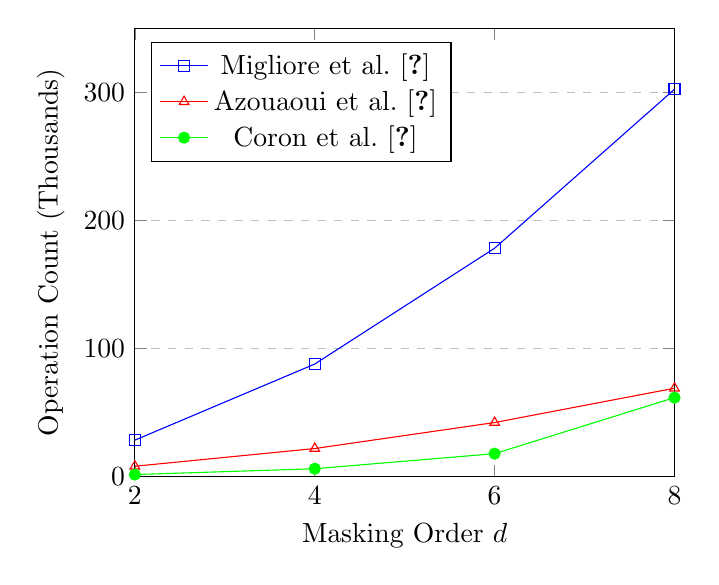
\begin{tikzpicture}
        \begin{axis}[
                xlabel={Masking Order $d$},
                ylabel={Operation Count (Thousands)},
                xmin=2, xmax=8,
                ymin=0, ymax=350,
                xtick={2,4,6,8},
                ytick={0,100,200,300},
                legend pos=north west,
                ymajorgrids=true,
                grid style=dashed,
            ]

            \addplot[
                color=blue,
                mark=square,
            ]
            coordinates {
                    (2, 28.41)
                    (4, 87.82)
                    (6, 178.25)
                    (8, 302.35)
                };
            \addlegendentry{Migliore et al.\ \cite{Migliore19}}

            \addplot[
                color=red,
                mark=triangle,
            ]
            coordinates {
                    (2, 8.04)
                    (4, 21.86)
                    (6, 42.16)
                    (8, 68.94)
                };
            \addlegendentry{Azouaoui et al.\ \cite{Azouaoui22}}

            \addplot[
                color=green,
                mark=*,
            ]
            coordinates {
                    (2, 1.54)
                    (4, 6.10)
                    (6, 17.86)
                    (8, 61.60)
                };
            \addlegendentry{Coron et al.\ \cite{Coron23}}

        \end{axis}
    \end{tikzpicture}
    \caption{Operation Counts for Boolean-to-Arithmetic Conversion at Different Masking Orders}
    \label{fig:b2a_comparison}
\end{figure}

In Figure~\ref{fig:b2a_comparison}, Coron et al.'s method shows the lowest operation counts at smaller masking orders due to their optimized gadgets. However, the operation counts increase rapidly at higher masking orders, reflecting exponential complexity growth. Azouaoui et al.'s implementation maintains moderate operation counts even at higher masking orders, showing better scalability. Migliore et al.'s implementation shows a steeper increase in operation counts with higher masking orders, indicating less efficient scaling.

\section{Feasibility on Embedded Devices}

Feasibility on embedded devices depends on balancing security requirements with performance constraints. Table~\ref{tab:feasibility} summarizes the feasibility considerations for each implementation.

\begin{table}[h]
    \centering
    \renewcommand{\arraystretch}{1.2} % Adjust row spacing
    \caption{Feasibility of Implementations on Embedded Devices}
    \begin{tabular}{l | p{10cm}} % Add a vertical line for separation
        \toprule
        \textbf{Implementation}            & \textbf{Feasibility Considerations}                                                                                                                     \\
        \midrule
        Migliore et al.\ \cite{Migliore19} & Practical for first-order masking on embedded devices due to moderate overhead and optimizations using a power-of-two modulus.                          \\
        Azouaoui et al.\ \cite{Azouaoui22} & Practical for higher-order masking up to $d=8$ on devices like ARM Cortex-M4, owing to optimized gadgets and performance gains from randomized signing. \\
        Coron et al.\ \cite{Coron23}       & Feasible at small masking orders; higher orders are less practical due to exponential complexity and resource constraints on embedded devices.          \\
        \bottomrule
    \end{tabular}
    \label{tab:feasibility}
\end{table}


Azouaoui et al.\ achieve feasible implementations even at higher masking orders by optimizing masking gadgets and leveraging randomized signing to reduce computational overhead. Conversely, Coron et al.'s implementation is limited to small masking orders on embedded devices due to increased complexity and resource requirements at higher orders.

\section{Implementation Techniques and Optimizations}

The specific techniques and optimizations employed significantly impact both security and performance. Table~\ref{tab:implementation_techniques} summarizes these techniques.

\begin{table}[h]
    \centering
    \renewcommand{\arraystretch}{1.2} % Adjust row spacing
    \caption{Implementation Techniques and Optimizations}
    \begin{tabular}{l | p{11cm}} % Add a vertical line for separation
        \toprule
        \textbf{Implementation}            & \textbf{Techniques and Optimizations}                                                                                                                                                                     \\
        \midrule
        Migliore et al.\ \cite{Migliore19} & Specialized algorithms for masking polynomial arithmetic; use of power-of-two modulus to simplify masking; focus on minimizing non-linear operations.                                                     \\
        Azouaoui et al.\ \cite{Azouaoui22} & Refined sensitivity analysis correcting previous flaws; new masking gadgets tailored for Dilithium; utilized PINI-compliant gadgets; leveraged randomized signing to avoid costly masked Keccak function. \\
        Coron et al.\ \cite{Coron23}       & Introduction of ShiftMod gadget; optimized Boolean-to-Arithmetic conversions; security proofs in the probing model; focused on efficiency at small masking orders.                                        \\
        \bottomrule
    \end{tabular}
    \label{tab:implementation_techniques}
\end{table}


Azouaoui et al.'s refined sensitivity analysis ensures that sensitive variables are protected, avoiding both insecurity and unnecessary overhead. Their new masking gadgets are specifically designed for Dilithium's operations, improving efficiency. Randomized signing allows them to bypass the performance bottleneck associated with masking the deterministic Keccak function.

\section{Trade-offs Between Security and Performance}

Balancing security and performance is a critical challenge in implementing side-channel resistant cryptographic algorithms, with each approach presenting unique trade-offs. Migliore et al.\ \cite{Migliore19} prioritize performance within a first-order masking framework, achieving basic side-channel resistance with moderate overhead. Their approach introduces a modification to the original Dilithium scheme by employing a power-of-two modulus to simplify masking, which improves efficiency but may affect standardization and interoperability.

In contrast, Azouaoui et al.\ \cite{Azouaoui22} emphasize a balance between high security and optimized performance, specifically through the use of higher-order masking combined with refined sensitivity analysis and tailored gadgets. Their approach avoids alterations to the standard Dilithium scheme, preserving compliance with existing standards, and achieves further performance gains by leveraging randomized signing. Randomized signing not only strengthens side-channel resistance but also minimizes the computational burden compared to deterministic alternatives, thereby reducing the attack surface.

Coron et al.\ \cite{Coron23} contribute by providing strong security proofs for their methods in the $t$-probing model, offering robust security assurances. They focus on improving efficiency at lower masking orders through innovative gadgets, such as their ShiftMod gadget. However, their approach faces scalability challenges: the exponential complexity associated with higher masking orders limits the practicality of their techniques on embedded devices.

In summary, Migliore et al.\ prioritize performance at the cost of modifying the scheme, Azouaoui et al.\ balance high-order security with optimized efficiency and standard compliance, and Coron et al.\ provide strong security at low masking orders but with scalability constraints. Each approach addresses the trade-off between security and performance differently, underscoring the importance of context-dependent choices in secure cryptographic implementations.

\section{Synthesis, Discussion, and Conclusion}

Our comparative analysis highlights that Azouaoui et al.'s implementation offers the best balance between high security and performance, particularly for higher-order masking. Their approach maintains compliance with the standard Dilithium scheme and is feasible on embedded devices, making it suitable for practical deployment.

Migliore et al.'s implementation is advantageous when only first-order masking is required and performance is a priority. However, the modification of the scheme by using a power-of-two modulus may present challenges in terms of standardization and interoperability.

Coron et al.'s implementation is valuable for its strong security proofs and efficiency at low masking orders. Nonetheless, the exponential increase in complexity at higher masking orders limits its practicality for applications requiring higher levels of side-channel resistance.

By examining the implementations across the key aspects of security level, performance metrics, feasibility on embedded devices, implementation techniques, and trade-offs, we conclude that Azouaoui et al.'s implementation provides the most practical solution for achieving high levels of side-channel resistance in Dilithium without compromising performance or standard compliance. Their use of refined sensitivity analysis, optimized masking gadgets, and randomized signing effectively addresses the challenges of masking Dilithium on embedded devices.
